%\documentclass[10pt,a4paper]{article}
\documentclass[12pt,a4paper]{article}
\usepackage{graphicx,amsmath}
%\usepackage{subfigure}
\usepackage{float}
\usepackage[german]{babel}
\usepackage[utf8]{inputenc}
\setcounter{secnumdepth}{4}
\usepackage[top=2cm, bottom=2.5cm, left=3cm, right=3cm]{geometry}
\usepackage{subcaption}
\begin{document}


%\title{Bachelorarbeit}
%\author{Richard Kullmann}
%\date{02.06.2017}

\thispagestyle{empty}
%\setcounter{page}{2}
\newpage
\tableofcontents
\thispagestyle{empty}
\newpage
\pagenumbering{arabic}

\section{Vergleich SNR-Theorie}
Das Signal-zu-Rausch Verhältnis kann für ein Kosinus-Signal mit Stärke $\epsilon$ folgenderma"sen berechnet werden:
\begin{align*}
SNR=\frac{\epsilon ^2T}{4}\frac{|\chi(\omega)|^2}{S_0(\omega)}=\frac{\epsilon^2T|dr/dI|^2}{8\cdot D_{eff}}
\end{align*}
Wenn man die Ableitung der Feuerrate numerisch aus vorherigen Messungen bestimmt und den gemessenen Diffusionskoeffizienten verwendet, lässt sich eine gute Vorhersage des SNR treffen

\begin{figure}[H]
	\centering
	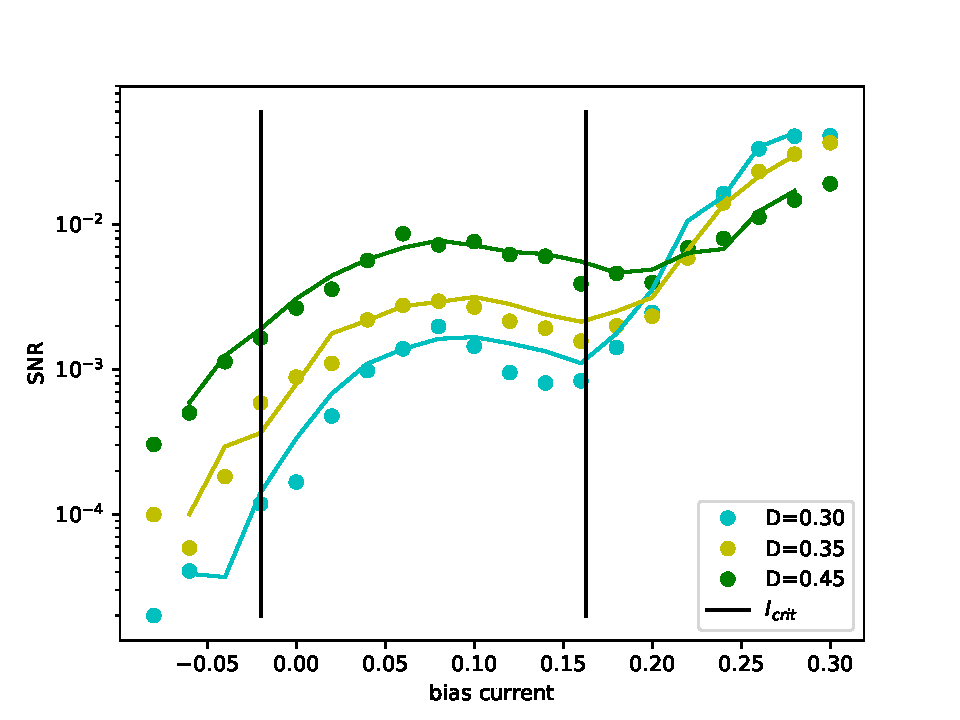
\includegraphics[scale=0.9]{snrangerealanameassp.pdf}
	\caption{Vergleich des SNR mit anderen Messwerten}
	\label{snrspike}
\end{figure}

Die mittleren Feuerraten nähern sich bei zunehmendem Bias-Strom $I$ der mittleren Feuerrate im burstenden Zustand an:
\begin{figure}[H]
	\centering
	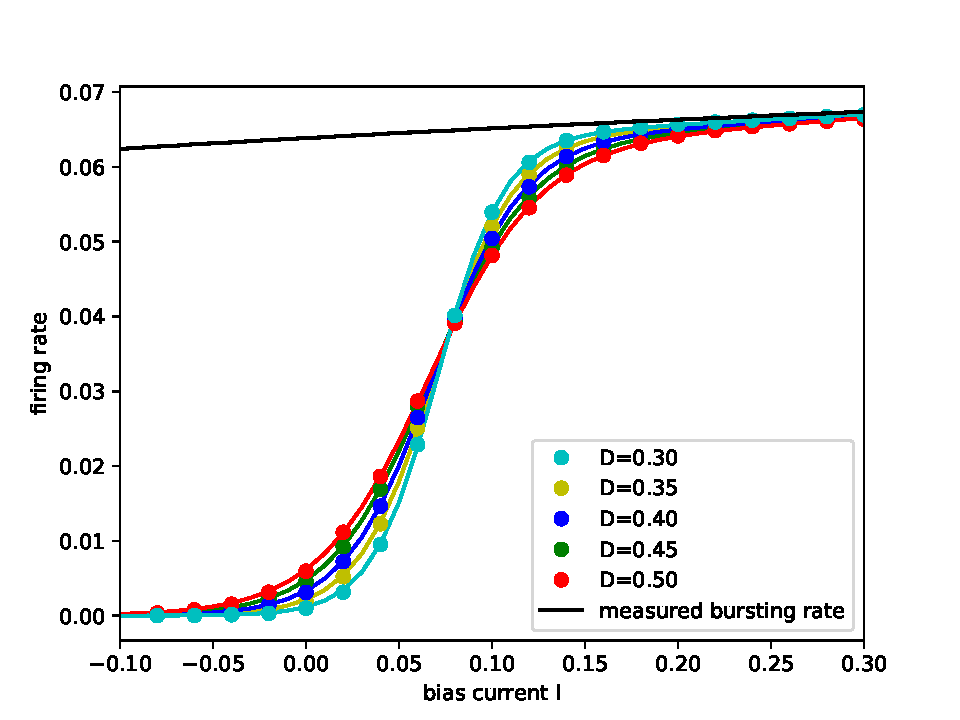
\includegraphics[scale=0.9]{ganaburst.pdf}
	\caption{Feuerraten und entsprechende Fits}
	\label{feuerrate}
\end{figure}

Das SNR des Spike Trains zeigt deutlich ausgeprägter das erwartete Verhalten:

\begin{figure}[H]
	\centering
	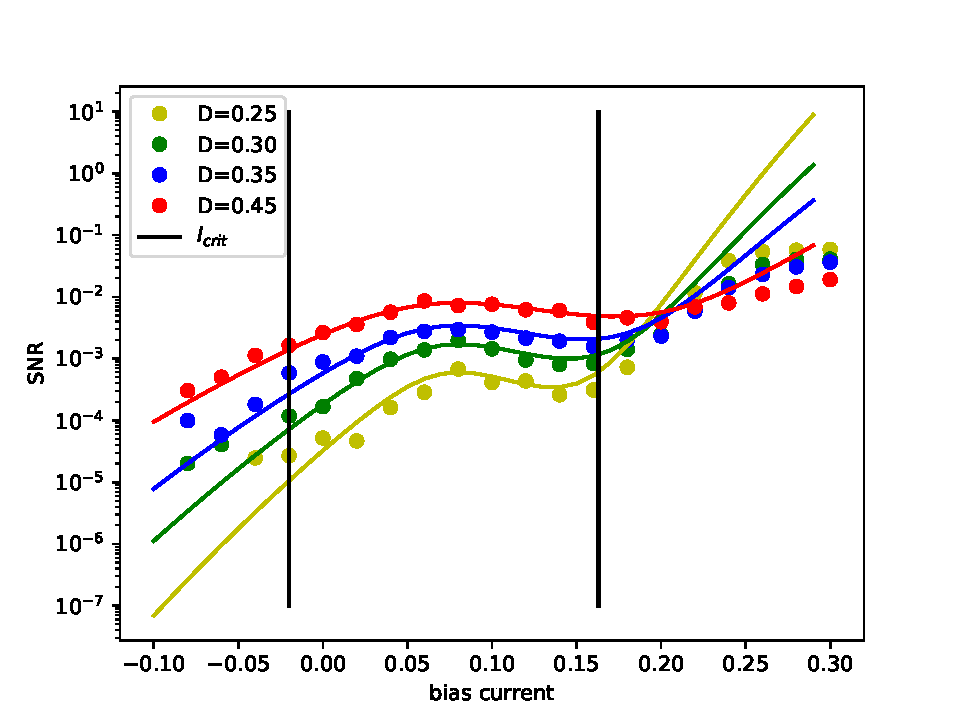
\includegraphics[scale=0.9]{snrautoreal13a25snrsp.pdf}
	\caption{Vergleich theoretisches und gemessenes Spektrum}
	\label{deltaspectrum}
\end{figure}
Es ist jedoch noch kein Zusammenhang mit dem kritischen Strom erkennbar.\\
Eine Vorhersage der Messwerte lässt sich jedoch auch auf andere Arten treffen. Versucht man, das SNR vorherzusagen, ohne die Potentialbarrieren zu fitten, bekommt man zwar keine glatten Kurven, aber immer noch eine gute Übereinstimmung:
\begin{figure}[H]
	\centering
	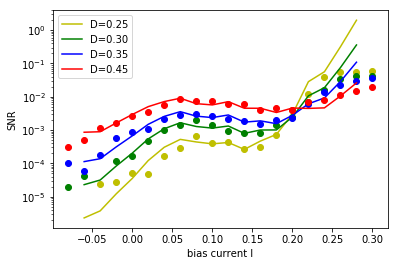
\includegraphics[scale=0.9]{snrdudionly.png}
	\caption{Vergleich SNR mit Theorie, wobei hier die Ableitung der Potenziale numerisch bestimmt wurde}
	\label{dudiplot}
\end{figure}

\begin{figure}[H]
	\centering
	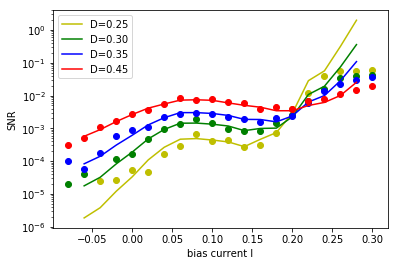
\includegraphics[scale=0.9]{snrdrcomp.png}
	\caption{Vergleich SNR mit Theorie, wobei hier in die Ableitung auch die numerische Ableitung der Vorfaktoren einging}
	\label{dcomp}
\end{figure}

\end{document}